% !TEX program = xelatex % 指定排版引擎为 xelatex。
% !BIB program = biber % 指定 bib 数据后端处理程序为 biber。
\documentclass[11pt,a4paper,twoside,UTF8,titlepage,fontset=none]{ctexart} % 指定 ctexart 文档类,设置基本字号为 11pt,a4 大小,双面排版,显式指定文档为 UTF-8 编码,令 \maketitle 命令可以生成单独的标题页(否则不单独成页),fontset 设置为 none 以关闭 Redefining CJKfamily xxx 的警告(不影响下面的字体设定)。

\usepackage{syntonly}
%\syntaxonly % 用以快速编译以排查错误,不生成 DVI 或 PDF。

%! ----------------------------------------------------------------
%! 创建文档时必须要设定的参数。
%! 使用 newcommand 定义空命令时,后面的大括号不建议省略(若无空行时,则会把下一行的内容当作命名所定义内容处理)。
%! ----------------------------------------------------------------
\newcommand{\ArticleClass}{} % 定义空命令,用以判断文档类。art 类时保留该命令,非 art 类请注释掉。
\newcommand{\DocumentTitle}{文档标题测试}
\newcommand{\DocumentCreatedDate}{2020.1.28}

%! ----------------------------------------------------------------
%! 相关信息在标题页和页脚等处均有显示。设定后一般不作修改。
%! ----------------------------------------------------------------
\newcommand{\AuthorName}{Mr. Kin}
\newcommand{\AuthorEmail}{im.misterkin@gmail.com}
\newcommand{\AuthorBlog}{https://mister-kin.github.io/}

%! ----------------------------------------------------------------
%! 一些命令定义和环境定义。
%! ----------------------------------------------------------------
\newcommand{\collections}{} % 主文件中定义汇总文件命令,以方便拆分源文件进行编写,子文件会有相关判断语句。

% 定义 intro 环境,用以章节开头的文字介绍。排版上比普通正文多缩进两个文字。
\newenvironment{intro}{\narrower\sffamily}{\par\vspace*{2ex plus 2.5ex minus 1.5ex}}

%! ----------------------------------------------------------------
%! 请不要随便修改以下导言区的代码
%! 除非你懂得你在干什么
%! ----------------------------------------------------------------
\usepackage{fontspec} % 调用 fontspec 宏包,以修改西文字体族。
\setmainfont{Source Serif Pro}
\setsansfont{Source Sans Pro}
\setmonofont{Source Code Pro}
\usepackage{xeCJK} %调用xeCJK宏包,以修改中文字体族。
\xeCJKsetup{AutoFakeSlant=true}  %设置伪斜体属性,以支持生成斜体中文字体(需置于中文字体设置之前)。
\setCJKmainfont{思源宋体}
\setCJKsansfont{思源黑体}
\setCJKmonofont{思源黑体}
% 针对文档类以相应设定全部标题为无衬线字体,即思源黑体(art 类无 chapter 命令,因此需分开设置)。
% 其中,为不改变原标题样式,使用 += 在原基础上追加命令。
\ifx\ArticleClass\undefined % 针对 rep 和 book 类。
\ctexset{
    part/format+=\sffamily,
    chapter/format+=\sffamily,
    section/format+=\sffamily,
    subsection/format+=\sffamily,
    subsubsection/format+=\sffamily,
    paragraph/format+=\sffamily,
    subparagraph/format+=\sffamily
}
\else % 针对 art 类。
\ctexset{
    part/format+=\sffamily,
    section/format+=\sffamily,
    subsection/format+=\sffamily,
    subsubsection/format+=\sffamily,
    paragraph/format+=\sffamily,
    subparagraph/format+=\sffamily
}
\fi
% 针对文档类以相应设定目录页中文字为无衬线字体,即思源黑体(art 类无 chapter 命令,因此需分开设置)。
\usepackage[subfigure]{tocloft} % 调用tocloft宏包,以修改目录排版样式。注意,tocloft 和 subfigure 宏包一起调用时,需指定 subfigure 参数。
\renewcommand{\cfttoctitlefont}{\huge\sffamily}
\renewcommand{\cftpartfont}{\bfseries\sffamily}
\ifx\ArticleClass\undefined % 针对 rep 和 book 类。
\renewcommand{\cftchapfont}{\bfseries\sffamily}
\renewcommand{\cftsecfont}{\sffamily}
\else % 针对 art 类。
\renewcommand{\cftsecfont}{\bfseries\sffamily}
\fi
\renewcommand{\cftsubsecfont}{\sffamily}
\renewcommand{\cftsubsubsecfont}{\sffamily}
\usepackage{tocbibind} % 调用宏包以添加目录本身和参考文献进目录中。
\usepackage[toc]{multitoc} % 调用 multitoc 宏包,以设置 toc 目录页多栏排版,默认双栏。
\usepackage[style=gb7714-2015]{biblatex} % 调用 biblatex 宏包,以排版参考文献。设置文献样式为符合中文文献著录标准 GB/T 7714-2015 的样式), 使用默认的后端程序 biber(其支持更好,包括 UTF-8 等,而 [backend=bibtex] 后端程序只支持 ascii 编码)。
\addbibresource{resources/reference.bib} % 指定参考文献数据库文件路径。
\usepackage{makeidx} % 调用 makeidx 宏包,以排版索引。
\makeindex % 开启索引收集
\usepackage[margin=1in]{geometry} % 调用 geometry 宏包,以设置页边距为 1 英寸。
\usepackage{xcolor} % 调用 xcolor 宏包,以支持生成颜色。
\usepackage{graphicx} % 调用 graphicx 宏包,以支持插入图片。
\graphicspath{{resources/images/},{resources/images/FollowMe/}} % 指定图片路径。
\usepackage{caption} % 调用 caption 宏包,以支持生成不带编号的图片等说明文字。
\usepackage{wrapfig} % 调用 wrapfig 宏包,以支持图文并排。
\usepackage{subfigure} % 调用 subfigure 宏包,以支持图片瀑布流排版。
\usepackage{tikz,tikz-qtree} % 调用 tikz 及其扩展宏包,以支持画图。
\usepackage{multicol} % 调用 multicol 宏包,以支持多栏排版。
\usepackage{enumitem} % 调用 emuitem 宏包,以设置列表环境。
\usepackage{multirow} % 调用 multirow 宏包,以支持纵向合并列表。
\usepackage{ulem} % 调用 ulem 宏包,以支持删除线等。
\usepackage{amsmath} % 调用 amsmath 宏包,以支持复杂的数学公式排版。
\usepackage[title,titletoc,header]{appendix} %调用 appendix,用 appendices 环境控制附录样式。
\usepackage{fancyhdr} % 为避免宏包冲突,一般在最后设置。调用 fancyhdr 宏包,以设置页眉页脚,文档风格设为:页眉为标题在左,页码在右;页脚为博客地址。
\pagestyle{fancy}
\fancyhf{}
\fancyhead[LO]{\sffamily \rightmark}
\fancyhead[LE]{\sffamily \leftmark}
\fancyhead[R]{\sffamily\bfseries \thepage}
\fancyfoot[C]{\ttfamily Author's Blog: \href{\AuthorBlog}{\color{black} \AuthorBlog}}
\renewcommand{\headrulewidth}{0.4pt}
\renewcommand{\footrulewidth}{0.4pt}
\usepackage{listings} % 指定listings,订制代码排版环境。
\lstset{
    basicstyle=\ttfamily, % 基本代码指定等宽字体。
    keywordstyle=\bfseries, % 关键字指定加粗。
    commentstyle=\ttfamily\slshape\color{gray}, % 注释指定灰色等宽斜体。
    stringstyle=\ttfamily,% 字符串指定等宽字体。
    %numbers=left, % 行号的位置在左边,启用后不方便复制代码。
    %numberstyle=\ttfamily, % 行号等宽字体。
    %xleftmargin=\parindent, % 代码左边框起始位置(启用行号时建议启用这个)。
    %frame=trBL, % 代码框类型,t下,r右,b下,l左,大写时为两条线。
    %frameround=fttt, % 控制代码框是否为圆角。
    frameshape={{ryrynyyyy}{yny}{yny}{ryrynyyyy}}, % 控制边框样式,上下边是每三个字母段控制一条边框。
    backgroundcolor=\color{gray!5}, % 代码框背景颜色:5% 的灰色。
    breaklines=true,% 代码过长时则换行。
    gobble=8, % 去掉代码前多余的缩进。
}
\usepackage[bookmarks=true]{hyperref} % 为不引起宏包冲突,hyperref 宏包一般在最后调用。调用 hyperref 宏包,bookmark 参数只能在调用时指定。
\hypersetup{
    colorlinks=true, % 设置超链接文件带颜色。
    bookmarksopen=true, % 书签展开。
    bookmarksnumbered=true, % 书签带章节编号。
    CJKbookmarks=true, % CJK 必设参数。
    unicode, % UTF-8 编码必设参数。
    pdftitle={\DocumentTitle}, % 设置 PDF 文件属性标题。
    pdfauthor={\AuthorName}, % 设置 PDF 文件属性作者。
    pdfstartview=FitH % 默认适合宽度显示。
}

    \title{\hypertarget{title}{\sffamily\huge\textbf{\DocumentTitle}}}
    \ifx\ArticleClass\undefined % 针对 rep 和 book 类。
    \addcontentsline{toc}{chapter}{标题页}
    \else % 针对 art 类。
    \addcontentsline{toc}{section}{标题页}
    \fi
    \author{\sffamily Written by \AuthorName \\ \sffamily Author's Blog: \href{\AuthorBlog}{\color{black} \AuthorBlog} \\ \sffamily Author's Email: \href{mailto:\AuthorEmail}{\color{black} \AuthorEmail}}
    \date{\sffamily 创建于\DocumentCreatedDate,修改于\number\year.\number\month.\number\day}

\begin{document}
    \phantomsection % 确保目录中的超链接指向正确的页码。
    \pdfbookmark[1]{标题页}{title} % 添加标题页书签。
    \pagenumbering{Roman} % 大写罗马字母样式页码。
    \maketitle % 生成标题页。
    \pagenumbering{roman} % 小写罗马字母样式页码。
    % !TEX root = OneClickSwitchLanguage.tex %指定主文件。
\ifx\collections\undefined
% !TEX program = xelatex %指定编译方式xelatex。
% !BIB program = biber %指定bib数据后台处理程序biber。
\documentclass[11pt,a4paper,UTF8,titlepage]{ctexart} %指定ctexart文档类,设置基本字号为11pt,a4大小,使用UTF-8编码保存,指定\maketitle生成单独的标题页。

\usepackage{syntonly}
%\syntaxonly %用来快速编译以排查错误,不生成DVI或PDF。
\usepackage[style=gb7714-2015]{biblatex} %调用biblatex宏包,设置参考文献样式(符合中文文献著录标准GB/T 7714-2015的样式),使用默认的后端程序biber(其支持更好,包括UTF-8等)放弃使用[backend=bibtex](只支持ascii编码)。
\addbibresource{resources/reference.bib} %加载参考文献数据库。
\usepackage{makeidx}
\makeindex %开启索引收集
\usepackage[margin=1in]{geometry} %调用geometry宏包,设置周围页边距为1英寸(为电子档设计,非打印)。
\usepackage{xcolor} %调用xcolor宏包,以支持扩展生成颜色。
\usepackage{fontspec} %调用fontspec宏包以更改西文字体族。
\setmainfont{Source Serif Pro}
\setsansfont{Source Sans Pro}
\setmonofont{Source Code Pro}
\usepackage{xeCJK} %调用xeCJK宏包以更改中文字体族。
\xeCJKsetup{AutoFakeSlant=true}  %设置xeCJK选项-伪斜体(需置于字体设置之前)。
\setCJKmainfont{思源宋体}
\setCJKsansfont{思源黑体}
\setCJKmonofont{思源等宽}
\usepackage{graphicx} %调用graphicx宏包,以支持插图。
\graphicspath{{resources/images/},{resources/images/FollowMe/}} %加载图片路径。
\usepackage{caption} %调用caption,支持不带编号的标题。
\usepackage{wrapfig} %调用wrapfig,支持图文排版。
\usepackage{subfigure} %调用subfigure宏包进行图片图片排版。
\usepackage{tikz,tikz-qtree} %调用tikz及其扩展宏包,以支持画图。
\usepackage[subfigure]{tocloft} %tocloft与subfigure宏包冲突,不能简单调用,tocloft需设置参数。
\usepackage{tocbibind} %调用宏包以添加目录本身和参考文献进目录中。
\usepackage{multicol} %调用multicol宏包以支持多栏排版。
\usepackage[toc]{multitoc} %调用multitoc宏包,设置toc目录页,默认双栏排版。
\usepackage{enumitem} %调用emuitem,以设置列表环境。
\usepackage{multirow} %调用multirow,以支持纵向合并列表。
%重订制目录命令。
\renewcommand{\tableofcontents}%
  {\chapter{\contentsname}%
  \@mkboth{\MakeUppercase\contentsname}{\MakeUppercase\contentsname}%
  \@makeschapterhead{\sourcecodename}%
  \@starttoc{toc}%
}
\usepackage{fancyhdr} %调用宏包,以设置页眉,统一格式:标题在左,页码在右。
\pagestyle{fancy}
\fancyhf{}
\fancyhead[LO]{\sffamily \rightmark}
\fancyhead[LE]{\sffamily \leftmark}
\fancyhead[ROE]{\bfseries \thepage}
\fancyfoot[COE]{\ttfamily \href{https://mister-kin.github.io}{个人博客:https://mister-kin.github.io}}
%定义intro环境。
\newenvironment{intro}{\narrower\sffamily}{\par\vspace*{2ex plus 2.5ex minus 1.5ex}}
\usepackage{listings} % 指定listings,订制代码排版环境
\lstset{
    basicstyle      = \ttfamily,                          % 基本代码指定等宽字体
    keywordstyle    = \bfseries,                          % 关键字指定加粗
    commentstyle    = \ttfamily\slshape\color{gray},      % 注释指定灰色等宽斜体
    stringstyle     = \ttfamily,                          % 字符串指定等宽字体
    %numbers        = left,                               % 行号的位置在左边,启用后不方便复制代码
    %numberstyle    = \ttfamily,                          % 行号等宽字体
    %xleftmargin    = \parindent,                         % 代码左边框起始位置(启用行号时建议启用这个)
    %frame          = trBL,                               % 代码框类型,t下,r右,b下,l左,大写时为两条线。
    %frameround     = fttt,                               % 控制代码框是否为圆角
    frameshape      = {{ryrynyyyy}{yny}{yny}{ryrynyyyy}}, % 控制边框样式,上下边是每三个字母段控制一条边框。
    backgroundcolor = \color{gray!5},                     % 代码框背景颜色:5%的灰色
    breaklines      = true,                               % 代码过长时则换行
    gobble          = 8,                                  % 去掉代码前的缩进
}
\usepackage{hyperref} %调用hyperref宏包
\hypersetup{
    colorlinks=true, %设置超链接文件带颜色
    bookmarks=true, %生成书签
    bookmarksopen=true, %书签展开
    bookmarksnumbered=true, %书签带章节编号
    CJKbookmarks=true, %cjk必设参数
    unicode, %utf-8编码必设参数
    pdftitle=标题, %设置PDF文件属性标题
    pdfauthor=Mr. Kin, %设置PDF文件属性作者
    pdfstartview=FitH %默认适合宽度显示
}

    \title{\hypertarget{title}{\textbf{标题}}}
    \addcontentsline{toc}{section}{标题页}
    \author{Written by Mr. Kin}
    \date{创建于2020.6.7,修改于\number\year.\number\month.\number\day}

\begin{document}
    \phantomsection %确保目录中的超链接指向正确的页码
    \pdfbookmark[1]{标题页}{title} %添加标题页书签
    \pagenumbering{Roman} %大写罗马样式页码
    \maketitle %生成标题页
    \pagenumbering{roman} %小写罗马样式页码
    {\centering \tableofcontents} %生成目录页
    \clearpage %新建页,分离上下两个样式页码的效果
    \pagenumbering{arabic} %阿拉伯样式页码
    \fi

    \phantomsection
    \section*{\bfseries \sffamily 关于作者}
    \addcontentsline{toc}{section}{关于作者}
    \markright{关于作者}

    \subsection*{\bfseries \sffamily 关于我}
    \begin{wrapfigure}[3]{L}{60pt}
        \vspace*{-20pt}
        \centering
        
\includegraphics{kin-logo}
    \end{wrapfigure}
    Mr. Kin,广东客家仁,程序猿,CG和游戏爱好者,一枚极客学生党。B站翻译up,个人up。不定时在B站直播日常:码代码,码博客,翻译,做视频,做教程。 ($\vartheta$$\bullet$\_$\bullet$)$\vartheta$ \hyperlink{follow}{\emph{(点击关注我!)}}

    \subsection*{\bfseries \sffamily 开源建设}

    \noindent 参与的开源软件中文化翻译

    \begin{itemize}
        \item krita文档:2018.8.5 - 2019.4.23
        \item \href{https://www.blendercn.org/5812.html?tdsourcetag=s_pctim_aiomsg}{Blender手册}:2019.7.20 - 2019.9.4 - 至今(\href{https://developer.blender.org/p/Mr_Kin/}{翻译维护})
    \end{itemize}

    \subsection*{\bfseries \sffamily \hypertarget{contact}{联系方式}}
    \vspace*{-1ex}
    \noindent {\footnotesize \emph{\color{red}注:联系时请注明身份,谢谢!}}

    \begin{itemize}
        \item QQ:\href{tencent://AddContact/?fromId=45&fromSubId=1&subcmd=all&uin=2312463626&website=www.oicqzone.com}{2312463626}\emph{\color{red}(点击号码加好友)}
        \item 邮箱:2312463626@qq.com ;moyu1355@gmail.com
    \end{itemize}

    \subsection*{\bfseries \sffamily \hypertarget{follow}{关注渠道}}
    \vspace*{-1ex}
    \noindent {\footnotesize\emph{\color{red}注:点击文字即可跳转关注!}}
    \vspace*{-2ex}

    \begin{figure}[htbp]
        \centering
        
\includegraphics[scale=0.2]{WechatOfficialAccounts.png}
    \end{figure}
    \vspace*{-4ex}

    \begin{figure}[htbp]
        \centering
        \begin{minipage}[t]{0.2\textwidth}
            \centering
            \setlength{\abovecaptionskip}{1pt}
            \caption*{\href{https://mister-kin.github.io}{博客 - Blog}}
            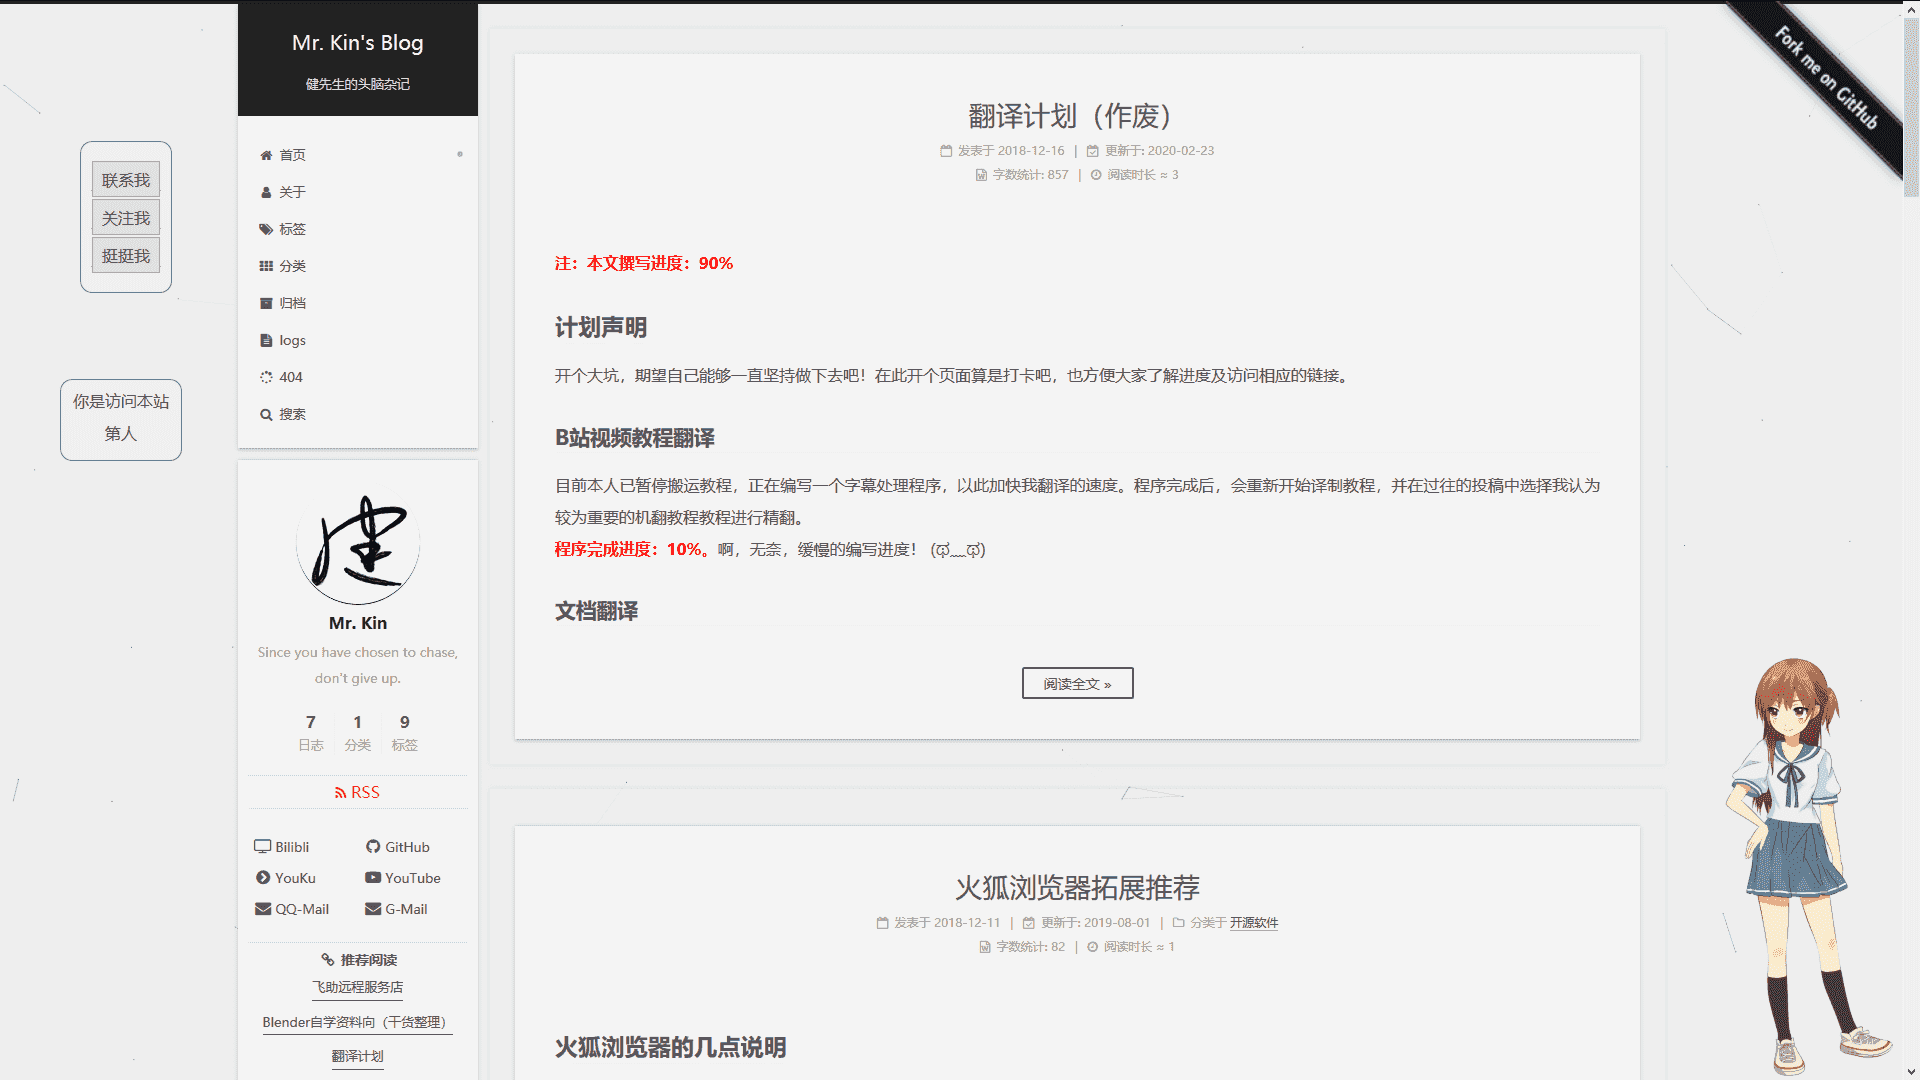
\includegraphics[scale=0.055]{Blog}
        \end{minipage}
        \qquad
        \begin{minipage}[t]{0.2\textwidth}
            \centering
            \setlength{\abovecaptionskip}{1pt}
            \caption*{\href{https://github.com/mister-kin}{Github}}
            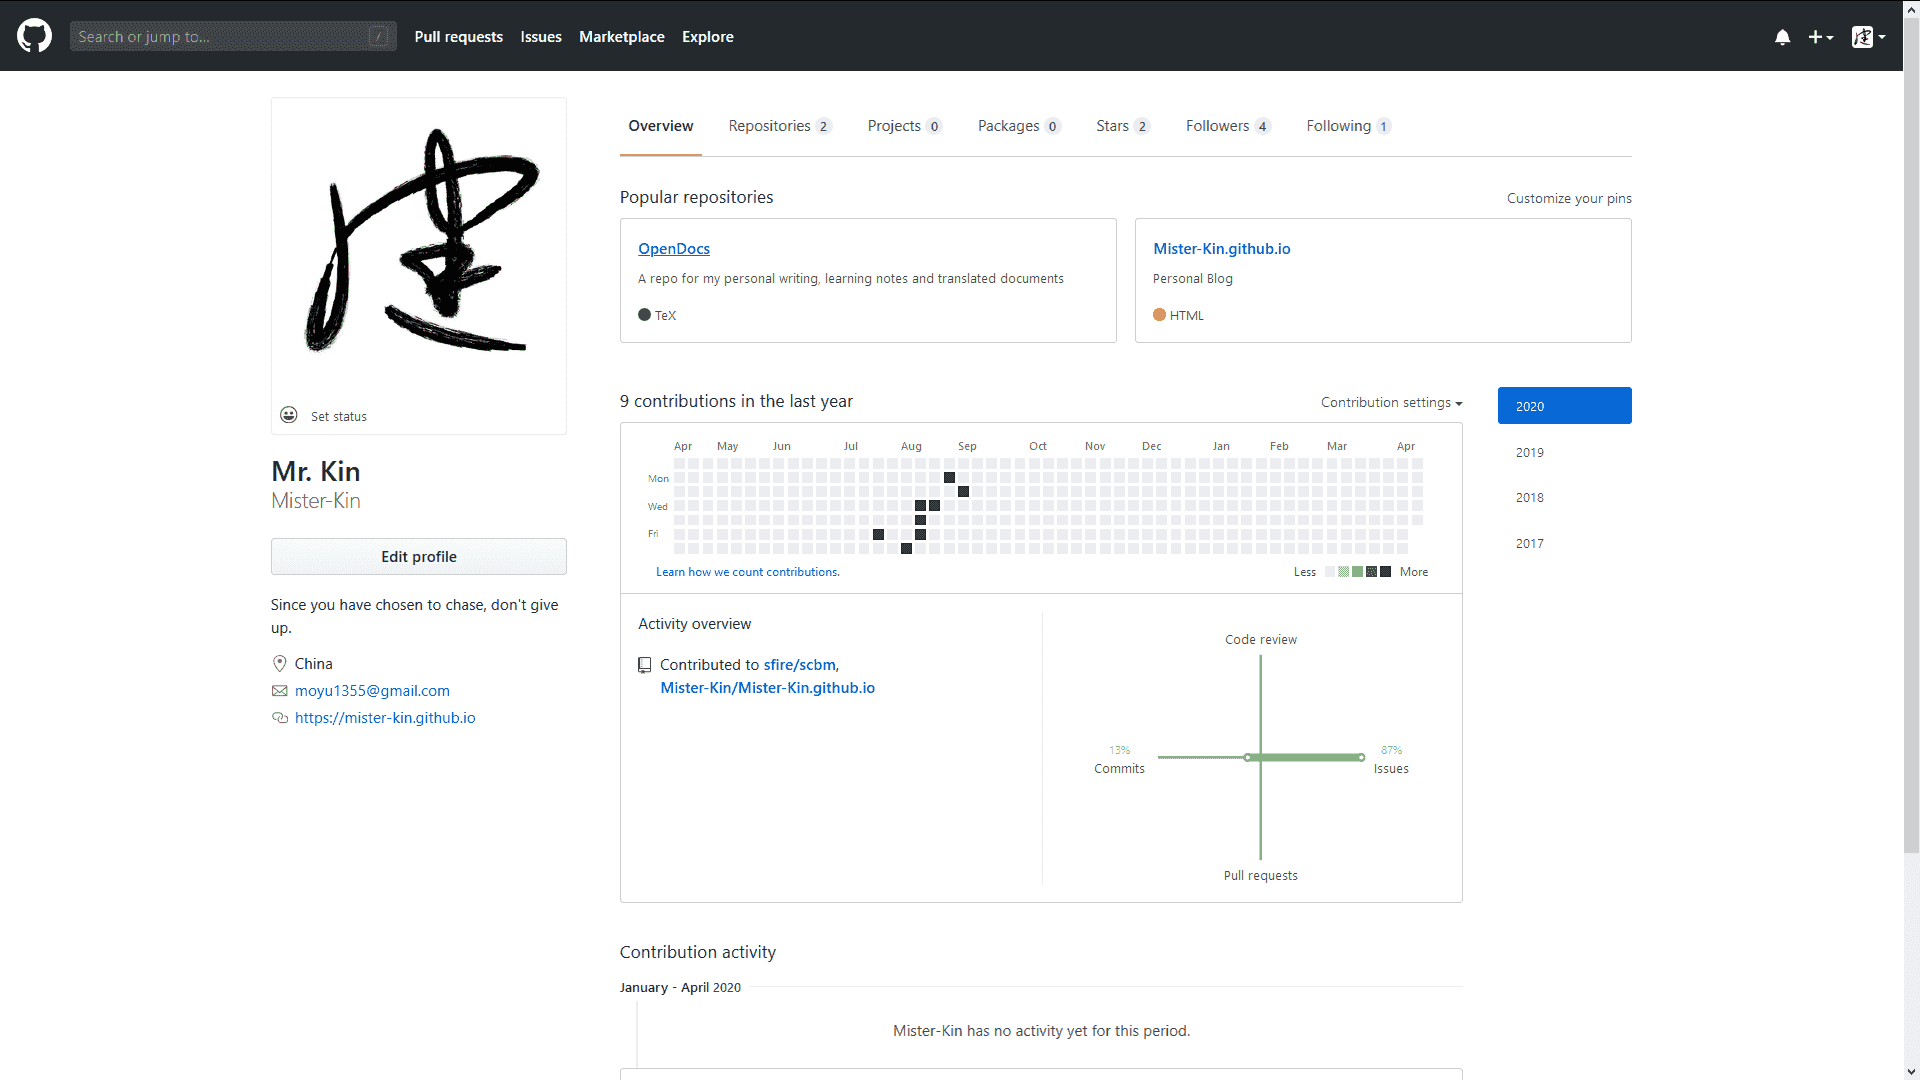
\includegraphics[scale=0.055]{Github}
        \end{minipage}
        \qquad
        \begin{minipage}[t]{0.2\textwidth}
            \centering
            \setlength{\abovecaptionskip}{1pt}
            \caption*{\href{https://weibo.com/6270111192/profile?topnav=1&wvr=6&is_all=1}{微博 - Weibo}}
            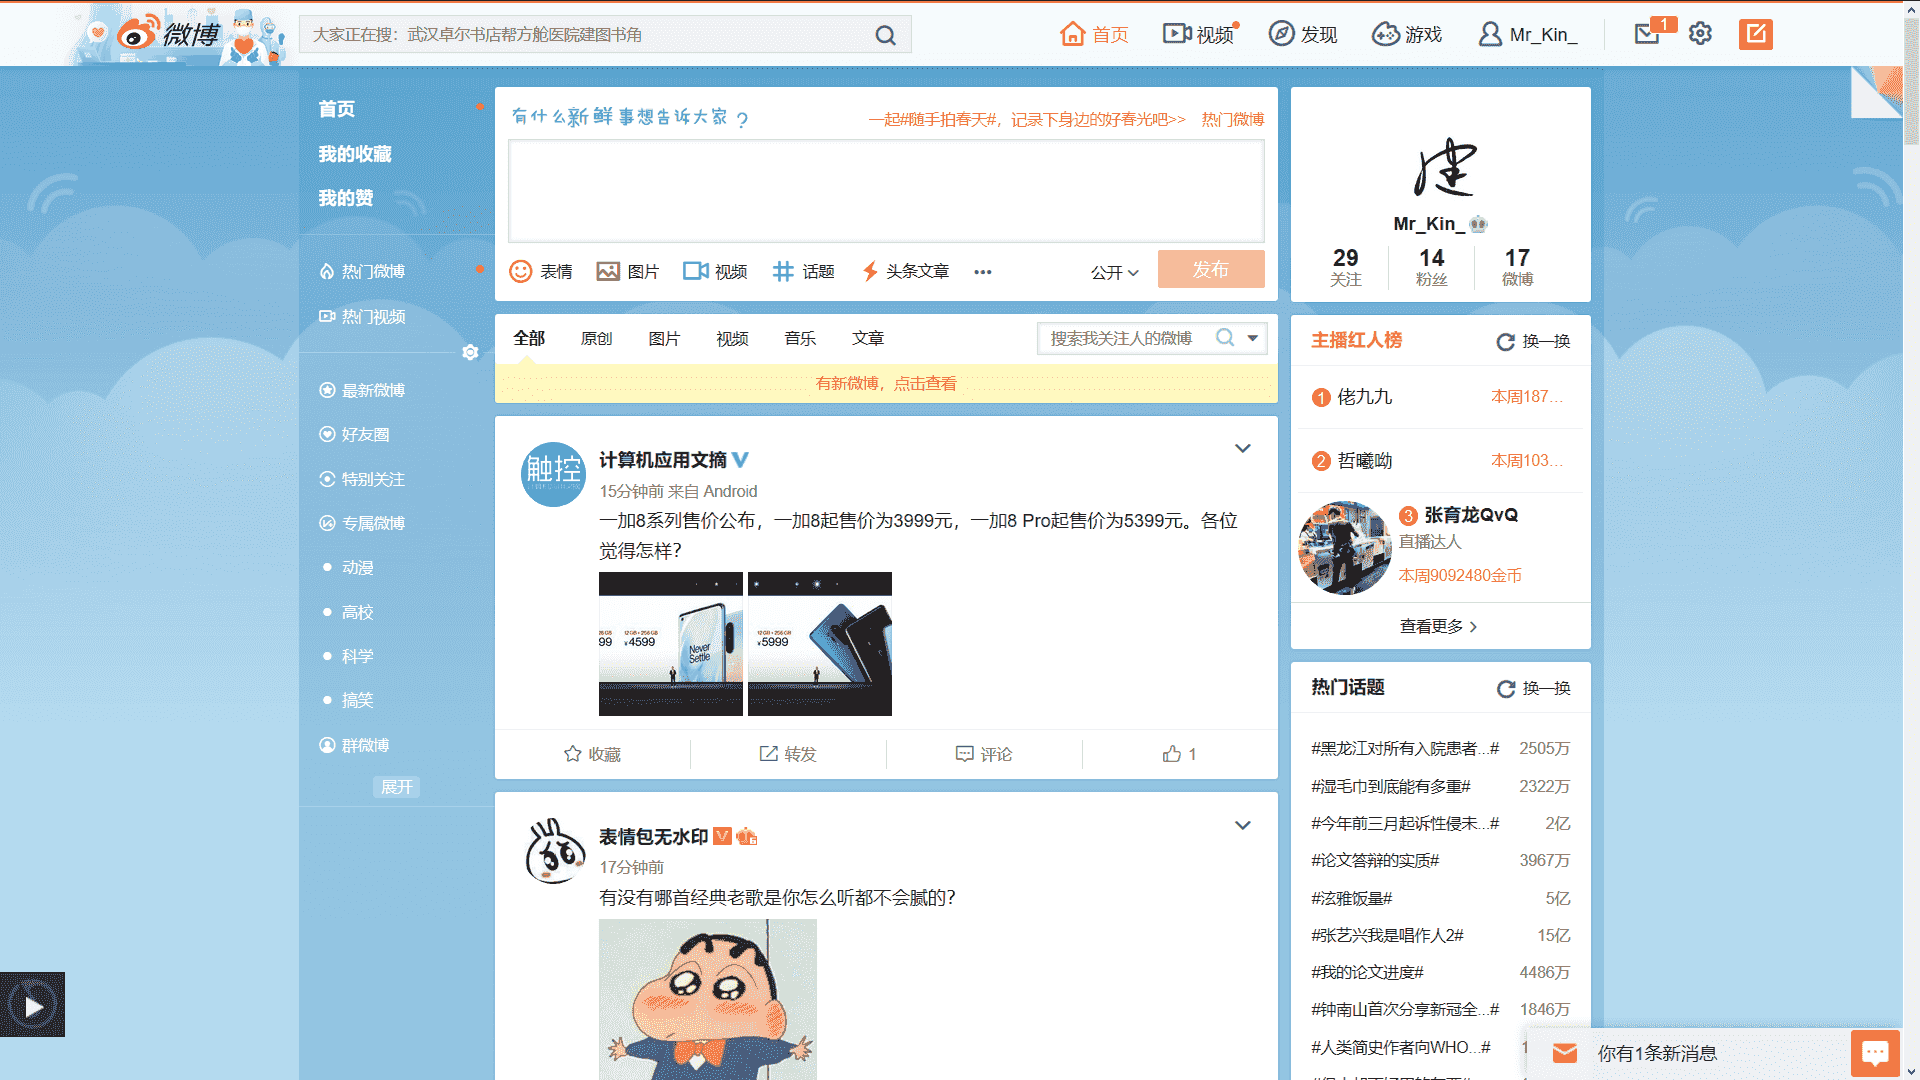
\includegraphics[scale=0.055]{Weibo}
        \end{minipage}
        \qquad
        \begin{minipage}[t]{0.2\textwidth}
            \centering
            \setlength{\abovecaptionskip}{1pt}
            \caption*{\href{https://www.zhihu.com/people/drwu-94}{知乎 - Zhihu}}
            
\includegraphics[scale=0.055]{Zhihu}
        \end{minipage}
        \qquad

        \begin{minipage}[t]{0.2\textwidth}
            \centering
            \setlength{\abovecaptionskip}{1pt}
            \setlength{\belowcaptionskip}{10pt}
            \caption*{\href{http://space.bilibili.com/17025250?}{B站 - Bilibili}}
            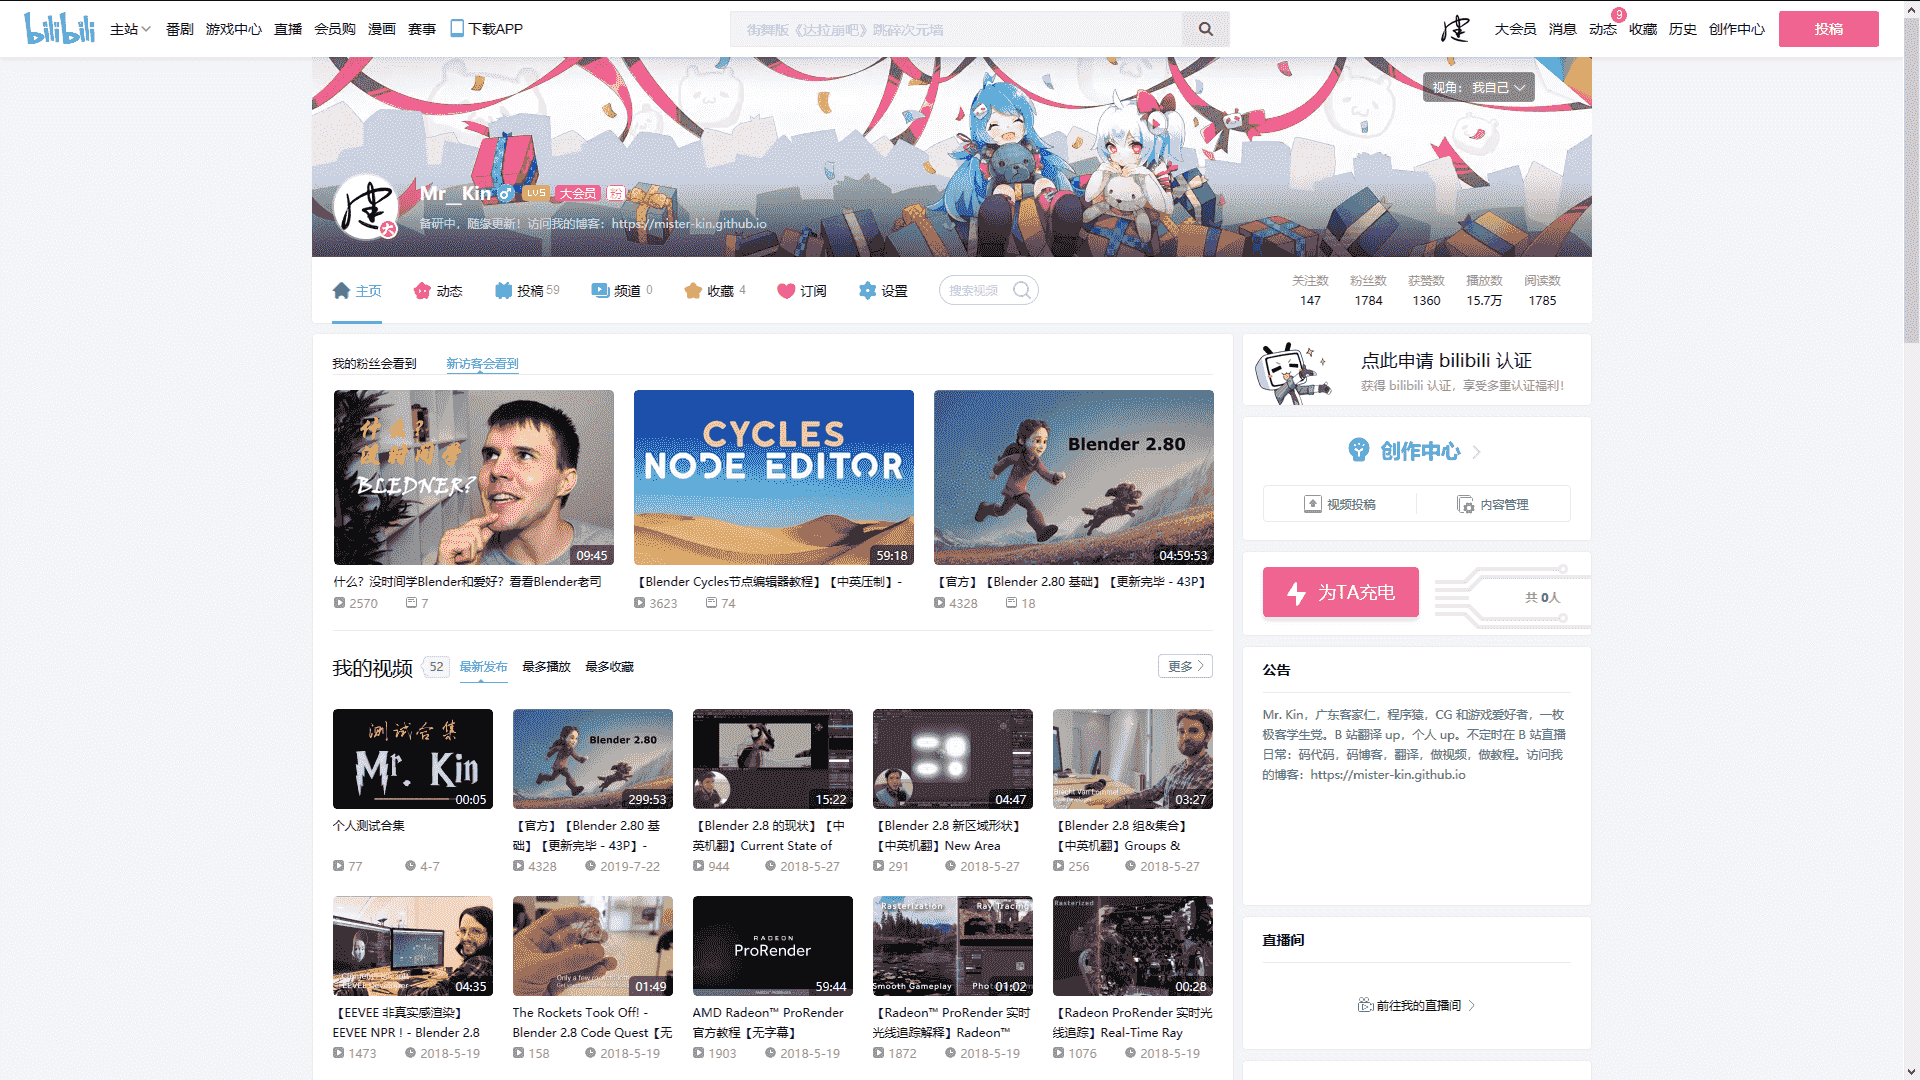
\includegraphics[scale=0.055]{Bilibili}
        \end{minipage}
        \qquad
        \begin{minipage}[t]{0.2\textwidth}
            \centering
            \setlength{\abovecaptionskip}{1pt}
            \setlength{\belowcaptionskip}{10pt}
            \caption*{\href{http://i.youku.com/i/UNjA3MTk5Mjgw?spm=a2hzp.8253869.0.0}{优酷 - Youku}}
            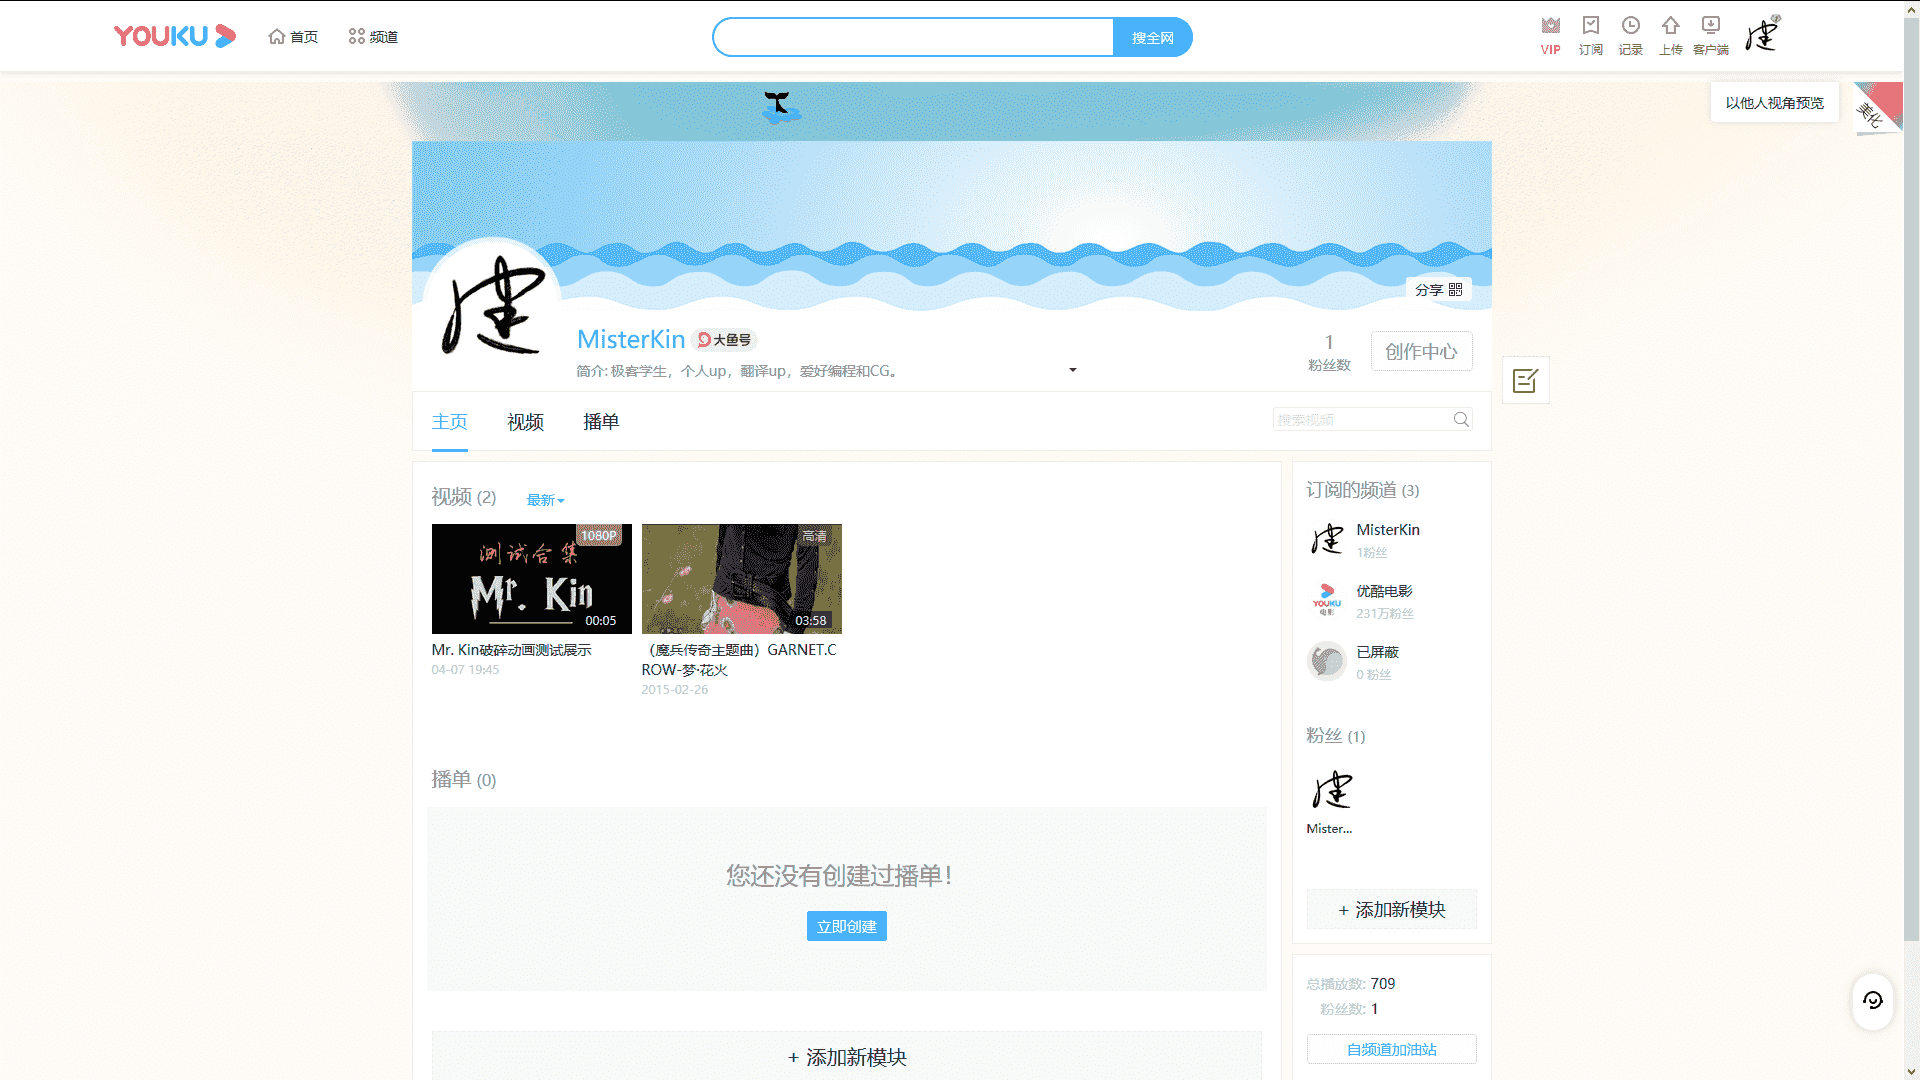
\includegraphics[scale=0.055]{Youku}
        \end{minipage}
        \qquad
        \begin{minipage}[t]{0.2\textwidth}
            \centering
            \setlength{\abovecaptionskip}{1pt}
            \setlength{\belowcaptionskip}{10pt}
            \caption*{\href{https://www.toutiao.com/c/user/835254071079053/\#mid=1663279303982091}{头条 - Headline}}
            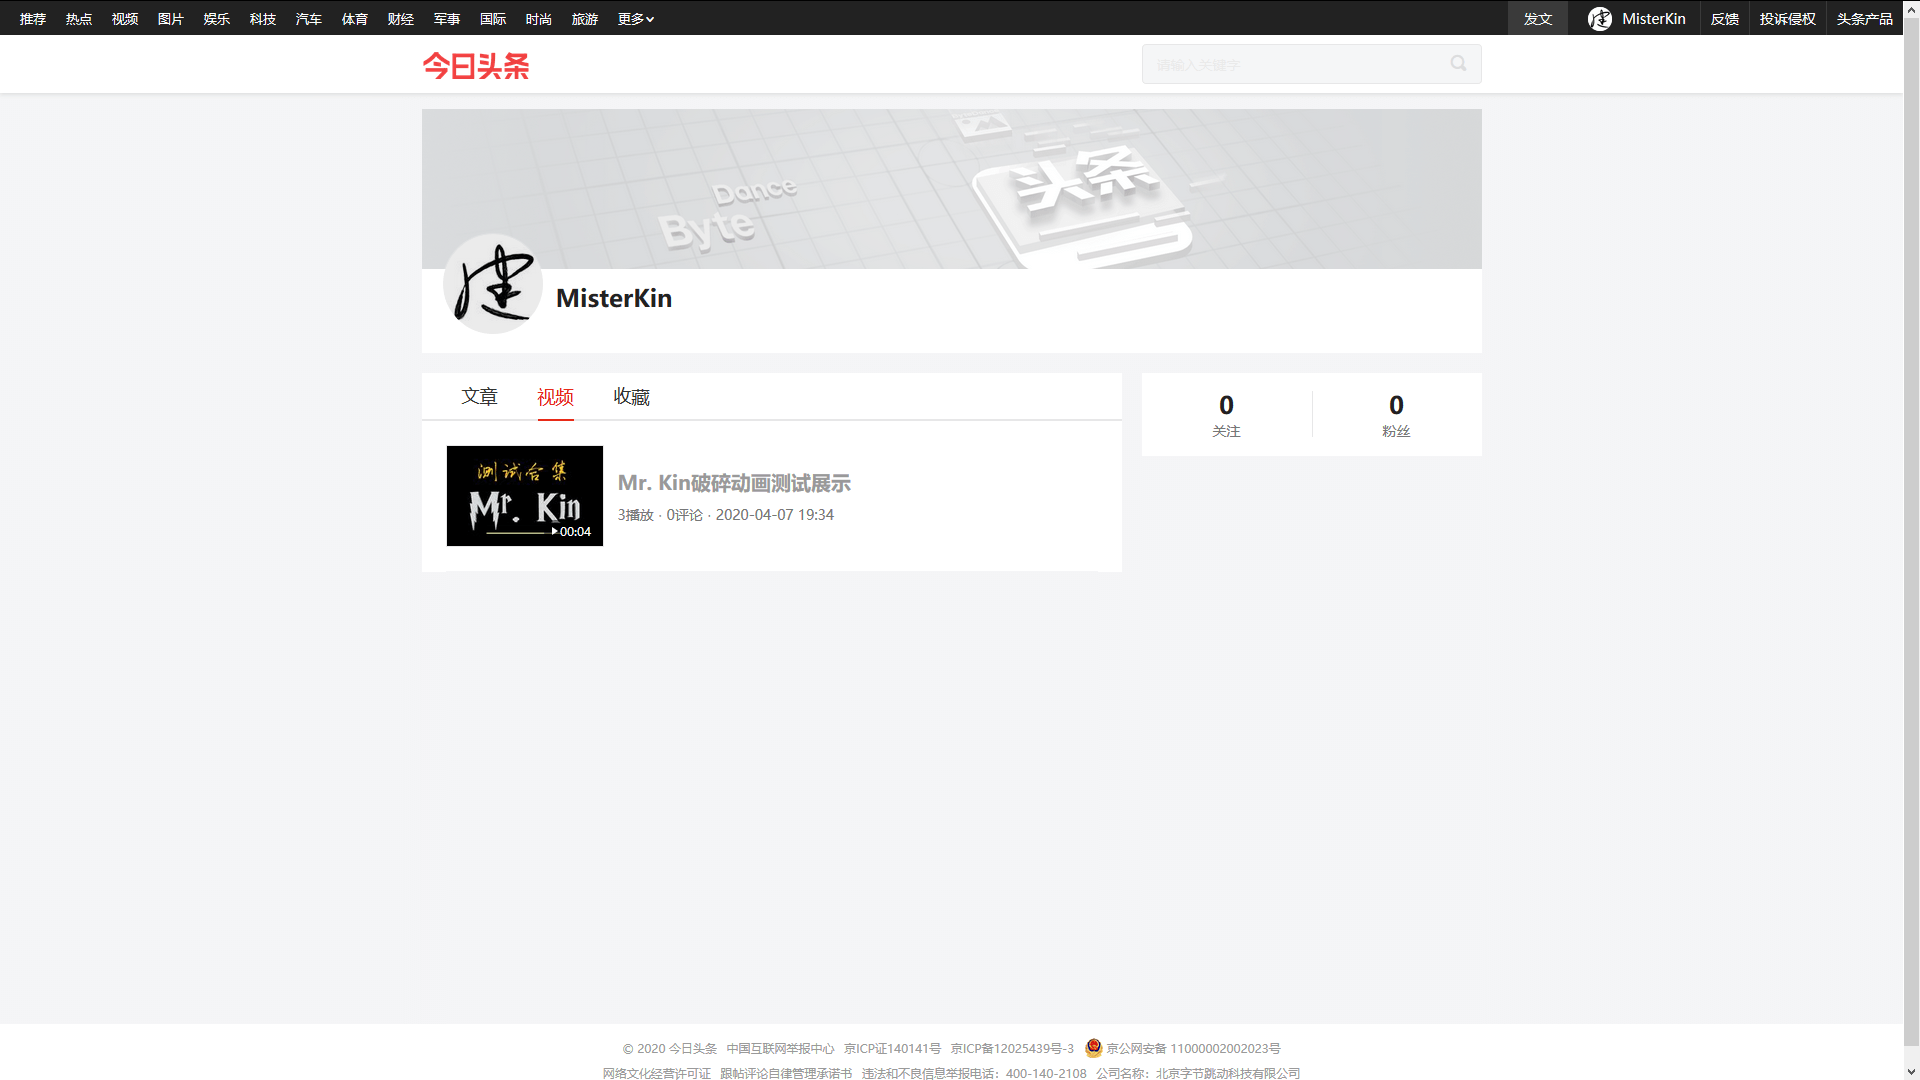
\includegraphics[scale=0.055]{Headline}
        \end{minipage}
        \qquad
        \begin{minipage}[t]{0.2\textwidth}
            \centering
            \setlength{\abovecaptionskip}{1pt}
            \setlength{\belowcaptionskip}{10pt}
            \caption*{\href{https://www.youtube.com/channel/UCNhtdG6whC5mlRDkrhQ0wLA?view_as=public}{油管 - Youtube}}
            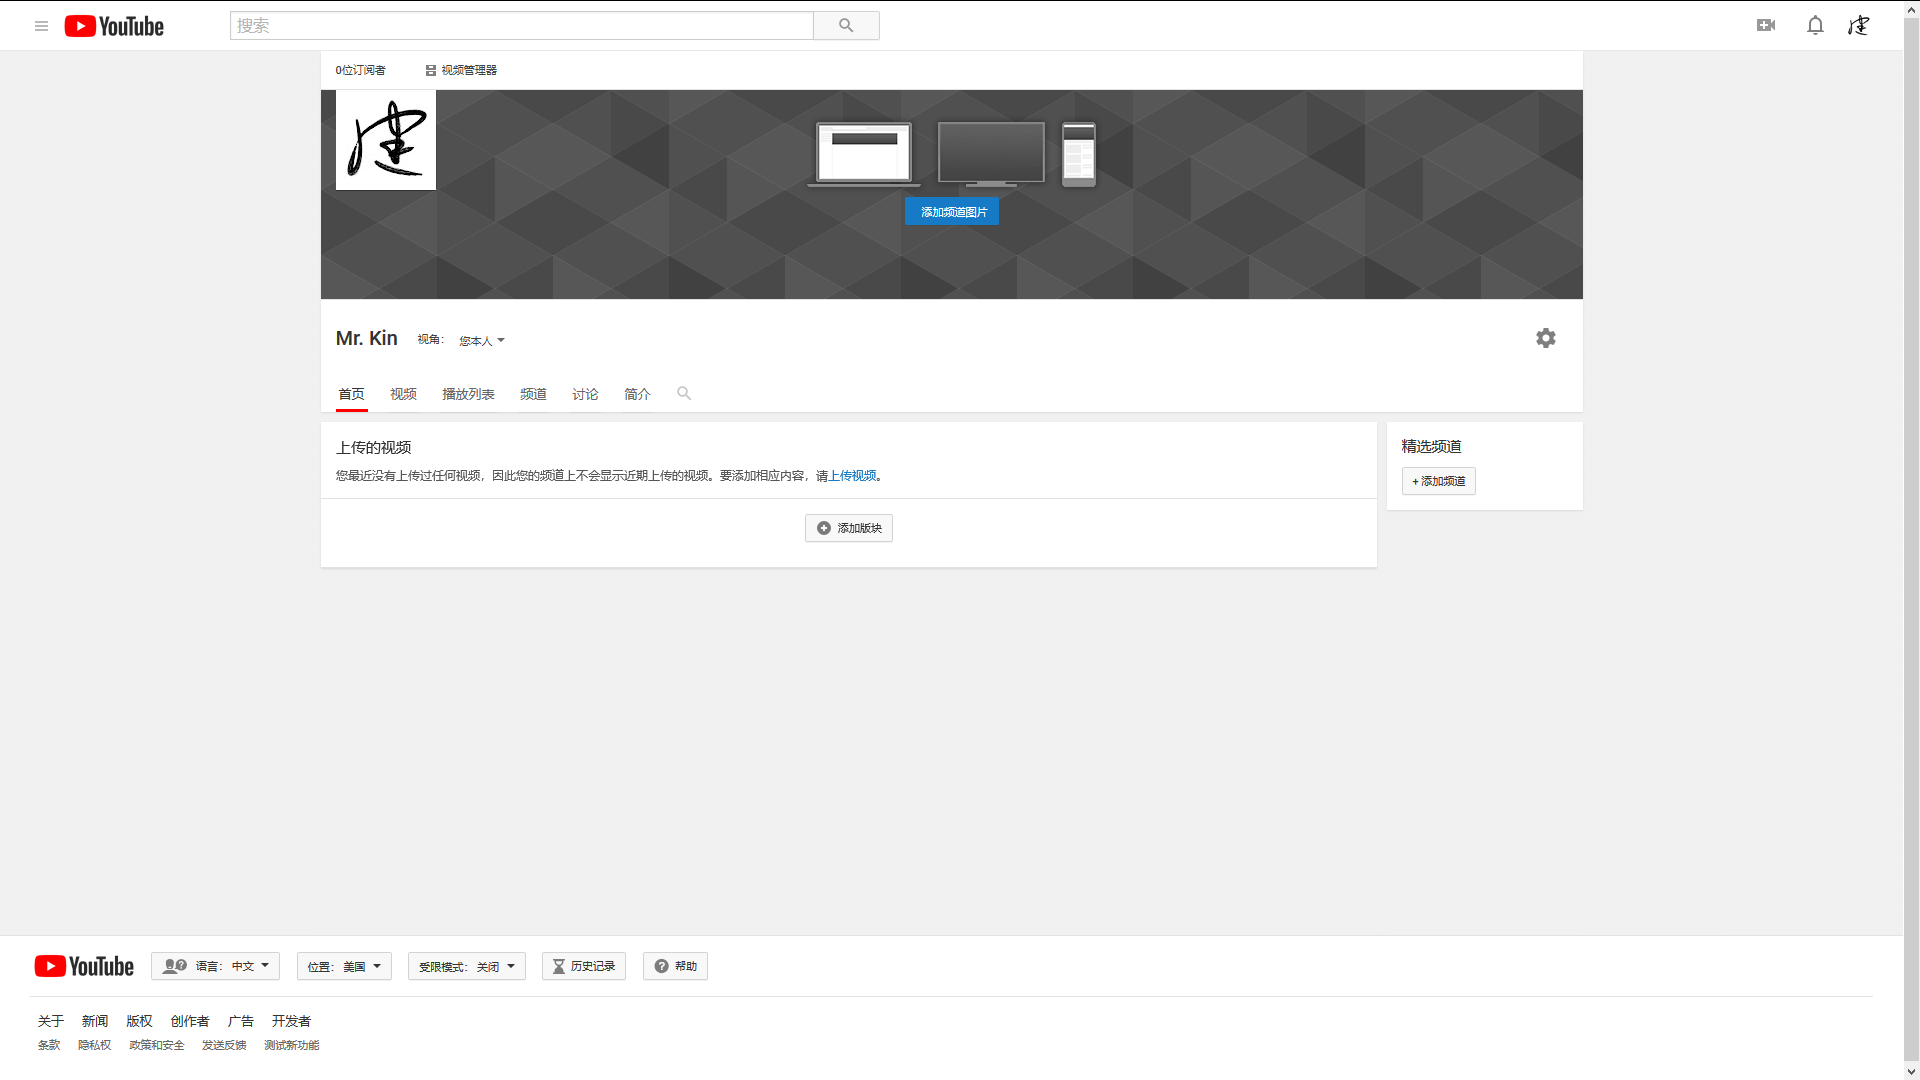
\includegraphics[scale=0.055]{Youtube}
        \end{minipage}
        \qquad
    \end{figure}

    \ifx\collections\undefined
    \printbibliography %生成参考文献排版。
    \addcontentsline{toc}{section}{参考文献} %添加参考文献进目录
    \clearpage %新建页,确保超链接跳转正确
    \phantomsection %确保目录中的超链接指向正确的页码
    \printindex %生成索引排版。
\end{document}
    \fi
 % 关于页面。
    \phantomsection
\begin{center}
    {\bfseries\sffamily\Large 版权声明}
\end{center}
\addcontentsline{toc}{chapter}{版权声明}

\noindent 作者:Mr. Kin \\
\DetectToksEmpty\LinkBlogPost
\ifToksEmpty
博文链接:链接暂空\\
\else
博文链接:\href{\the\LinkBlogPost}{跳转博文页}\\
\fi
\DetectToksEmpty\LinkPDFSource
\ifToksEmpty
PDF及LaTex源码链接:链接暂空\\
\else
PDF及LaTex源码链接:\href{\the\LinkPDFSource}{跳转PDF及LaTex源码页}\\
\fi
\DetectToksEmpty\LinkVideo
\ifToksEmpty
\else
相关视频创作链接:\href{\the\LinkVideo}{跳转视频页}\\
\fi
许可协议:本作品的所有内容,除个人设计创作的图像(如logo等)和相关的视频创作及其他特别声明外,均采用\href{https://creativecommons.org/licenses/by-nc-sa/4.0/deed.zh}{知识共享\ 署名-非商业性使用-相同方式共享 4.0 国际许可协议}进行发布。版权 © Mr. Kin,保留所有权利。
\includegraphics[scale=.4]{CC-BY-NC-SA}\\*[1.3ex]
\begin{tabular}{|*{3}{p{0.306\textwidth}|}}
    \hline
    \textsf{\bfseries 允许} & \textsf{\bfseries 限制} & \textsf{\bfseries 条件} \\
    \hline
    \vspace{-8pt}{\color{green}√} 修改 & \vspace{-8pt}{\color{red}×} 商标使用 & \vspace{-8pt}{\color{blue}$\odot$} 保留原署名 \\[-12pt]
    {\color{green}√} 分发 & {\color{red}×} 专利使用 & {\color{blue}$\odot$} 状态变更说明 \\[-12pt]
    {\color{green}√} 个人使用 & {\color{red}×} 商业使用 & {\color{blue}$\odot$} 相同的许可和版权声明 \\
    \hline
\end{tabular}
\\*[1.3ex]
\emph{注:若想对本作品进行转载、引用亦或是进行二次创作时,请详细阅读上述相关协议内容(若不理解,请点击链接跳转阅读)。为保障本人权利,对于违反者,本人将依法予以处理!望周知!——Mr. Kin}

\begin{center}
    {\bfseries\sffamily\Large 勘误声明}
\end{center}

虽本人写作时已尽力保证其内容的正确性,但因个人知识面和经验的局限性以及计算机技术等相关技术日新月异,本作品内容或存在一些错误之处。还望诸君发现错误后能够\hyperlink{contact}{联系我}以更正错误,不胜感激!——Mr. Kin

\begin{center}
    {\bfseries\sffamily\Large 侵权声明}
\end{center}

若本作品采用的第三方内容侵犯了你的版权,请与我\hyperlink{contact}{联系}进行处理,谢谢!——Mr. Kin

\begin{center}
    {\bfseries\sffamily\Large 第三方开源许可声明}
\end{center}

\noindent 本作品使用的第三方开源产品有:
\begin{multicols}{2}
\begin{itemize}
    \item \href{https://github.com/adobe-fonts}{Adobe Fonts}: \href{https://github.com/adobe-fonts/source-serif-pro/blob/release/LICENSE.md}{OFL v1.1}
    \item \href{https://tug.org/texlive/}{Tex Live}: \href{https://tug.org/texlive/copying.html}{TeX Live Licensing}
    \item \href{https://code.visualstudio.com/}{Visual Studio Code}: \href{https://github.com/Microsoft/vscode/blob/master/LICENSE.txt}{MIT}
    \item \href{http://ffmpeg.org/}{FFmpeg}: \href{http://ffmpeg.org/legal.html}{LGPL v2.1 / GPL v2}
    \item \href{https://krita.org/en/}{Krita}: \href{https://docs.krita.org/en/KritaFAQ.html?highlight=license#license-rights-and-the-krita-foundation}{Krita's GPL license}
    \item \href{https://inkscape.org/}{Inkscape}: \href{https://inkscape.org/about/license/}{GPL}
    \item \href{https://www.gimp.org}{GIMP}: \href{https://www.gimp.org/about/COPYING}{GPL}
    \item \href{https://www.blender.org}{Blender}: \href{https://www.blender.org/about/license/}{GPL}
    \item \href{https://www.audacityteam.org/}{Audacity}: \href{https://www.audacityteam.org/about/license/}{GPL v2}
    \item \href{https://handbrake.fr}{Handbrake}: \href{https://github.com/HandBrake/HandBrake/blob/master/LICENSE}{GPL v2}
\end{itemize}
\end{multicols}

\noindent 更多请点击查看\href{https://mister-kin.github.io/about/third-party-declaration/}{第三方声明页}!
 % 版权声明。
    {\centering \tableofcontents} % 生成目录页。
    \clearpage % 新建页,分离上下两个样式页码的效果。
    \pagenumbering{arabic} % 阿拉伯样式页码。

    % 正文
    % !TEX root = main.tex % 指定主文件。
\ifx\collections\undefined
% !TEX program = xelatex %指定编译方式xelatex。
% !BIB program = biber %指定bib数据后台处理程序biber。
\documentclass[11pt,a4paper,UTF8,titlepage]{ctexart} %指定ctexart文档类,设置基本字号为11pt,a4大小,使用UTF-8编码保存,指定\maketitle生成单独的标题页。

\usepackage{syntonly}
%\syntaxonly %用来快速编译以排查错误,不生成DVI或PDF。
\usepackage[style=gb7714-2015]{biblatex} %调用biblatex宏包,设置参考文献样式(符合中文文献著录标准GB/T 7714-2015的样式),使用默认的后端程序biber(其支持更好,包括UTF-8等)放弃使用[backend=bibtex](只支持ascii编码)。
\addbibresource{resources/reference.bib} %加载参考文献数据库。
\usepackage{makeidx}
\makeindex %开启索引收集
\usepackage[margin=1in]{geometry} %调用geometry宏包,设置周围页边距为1英寸(为电子档设计,非打印)。
\usepackage{xcolor} %调用xcolor宏包,以支持扩展生成颜色。
\usepackage{fontspec} %调用fontspec宏包以更改西文字体族。
\setmainfont{Source Serif Pro}
\setsansfont{Source Sans Pro}
\setmonofont{Source Code Pro}
\usepackage{xeCJK} %调用xeCJK宏包以更改中文字体族。
\xeCJKsetup{AutoFakeSlant=true}  %设置xeCJK选项-伪斜体(需置于字体设置之前)。
\setCJKmainfont{思源宋体}
\setCJKsansfont{思源黑体}
\setCJKmonofont{思源等宽}
\usepackage{graphicx} %调用graphicx宏包,以支持插图。
\graphicspath{{resources/images/},{resources/images/FollowMe/}} %加载图片路径。
\usepackage{caption} %调用caption,支持不带编号的标题。
\usepackage{wrapfig} %调用wrapfig,支持图文排版。
\usepackage{subfigure} %调用subfigure宏包进行图片图片排版。
\usepackage{tikz,tikz-qtree} %调用tikz及其扩展宏包,以支持画图。
\usepackage[subfigure]{tocloft} %tocloft与subfigure宏包冲突,不能简单调用,tocloft需设置参数。
\usepackage{tocbibind} %调用宏包以添加目录本身和参考文献进目录中。
\usepackage{multicol} %调用multicol宏包以支持多栏排版。
\usepackage[toc]{multitoc} %调用multitoc宏包,设置toc目录页,默认双栏排版。
\usepackage{enumitem} %调用emuitem,以设置列表环境。
\usepackage{multirow} %调用multirow,以支持纵向合并列表。
\usepackage{ulem} %调用ulem,以支持删除线等。
\usepackage{amsmath} %调用amsmath,以支持复杂的数学公式排版。
%重订制目录命令。
\renewcommand{\tableofcontents}%
  {\chapter{\contentsname}%
  \@mkboth{\MakeUppercase\contentsname}{\MakeUppercase\contentsname}%
  \@makeschapterhead{\sourcecodename}%
  \@starttoc{toc}%
}
\usepackage{fancyhdr} %调用宏包,以设置页眉,统一格式:标题在左,页码在右。
\pagestyle{fancy}
\fancyhf{}
\fancyhead[LO]{\sffamily \rightmark}
\fancyhead[LE]{\sffamily \leftmark}
\fancyhead[ROE]{\bfseries \thepage}
\fancyfoot[COE]{\ttfamily \href{https://mister-kin.github.io}{Author's Blog: https://mister-kin.github.io}}
%定义intro环境。
\newenvironment{intro}{\narrower\sffamily}{\par\vspace*{2ex plus 2.5ex minus 1.5ex}}
\usepackage{listings} % 指定listings,订制代码排版环境
\lstset{
    basicstyle      = \ttfamily,                          % 基本代码指定等宽字体
    keywordstyle    = \bfseries,                          % 关键字指定加粗
    commentstyle    = \ttfamily\slshape\color{gray},      % 注释指定灰色等宽斜体
    stringstyle     = \ttfamily,                          % 字符串指定等宽字体
    %numbers        = left,                               % 行号的位置在左边,启用后不方便复制代码
    %numberstyle    = \ttfamily,                          % 行号等宽字体
    %xleftmargin    = \parindent,                         % 代码左边框起始位置(启用行号时建议启用这个)
    %frame          = trBL,                               % 代码框类型,t下,r右,b下,l左,大写时为两条线。
    %frameround     = fttt,                               % 控制代码框是否为圆角
    frameshape      = {{ryrynyyyy}{yny}{yny}{ryrynyyyy}}, % 控制边框样式,上下边是每三个字母段控制一条边框。
    backgroundcolor = \color{gray!5},                     % 代码框背景颜色:5%的灰色
    breaklines      = true,                               % 代码过长时则换行
    gobble          = 8,                                  % 去掉代码前的缩进
}
\usepackage{hyperref} %调用hyperref宏包
\hypersetup{
    colorlinks=true, %设置超链接文件带颜色
    bookmarks=true, %生成书签
    bookmarksopen=true, %书签展开
    bookmarksnumbered=true, %书签带章节编号
    CJKbookmarks=true, %cjk必设参数
    unicode, %utf-8编码必设参数
    pdftitle=标题, %设置PDF文件属性标题
    pdfauthor=Mr. Kin, %设置PDF文件属性作者
    pdfstartview=FitH %默认适合宽度显示
}

    \title{\hypertarget{title}{\textbf{标题}}}
    \addcontentsline{toc}{section}{标题页}
    \author{Written by Mr. Kin \\ Author's Blog: \href{https://mister-kin.github.io}{\color{black} https://mister-kin.github.io} \\ Author's Email: im.misterkin@gmail.com}
    \date{创建于2020.1.28,修改于\number\year.\number\month.\number\day}

\begin{document}
    \phantomsection %确保目录中的超链接指向正确的页码
    \pdfbookmark[1]{标题页}{title} %添加标题页书签
    \pagenumbering{Roman} %大写罗马样式页码
    \maketitle %生成标题页
    \pagenumbering{roman} %小写罗马样式页码
    {\centering \tableofcontents} %生成目录页
    \clearpage %新建页,分离上下两个样式页码的效果
    \pagenumbering{arabic} %阿拉伯样式页码
    \fi

    \part{块标题测试}
    %\chapter{章标题测试}
    \section{节标题测试}
    \subsection{子节标题测试}
    \subsubsection{子子标题测试}
    \paragraph{段标题测试}
    测试
    \subparagraph{子段标题测试}
    测试

    {\rmfamily 思宋:测试 \textbf{粗体:测试} \textup{直立体:测试} { \itshape 意大利斜体:测试} { \slshape 倾斜体:测试}}

    {\sffamily 思黑:测试 \textbf{粗体:测试} \textup{直立体:测试} { \itshape 意大利斜体:测试} { \slshape 倾斜体:测试}}

    \ifx\collections\undefined
    \nocite{*} %不使用cite也能生成参考文献
    \printbibliography %生成参考文献排版。
    \addcontentsline{toc}{section}{参考文献} %添加参考文献进目录
    \clearpage %新建页,确保超链接跳转正确
    \phantomsection %确保目录中的超链接指向正确的页码
    \printindex %生成索引排版。
\end{document}
    \fi


    \nocite{*} % 不使用 cite 也能生成参考文献。
    \clearpage % 新建页,另起一页以生成文献。
    \printbibliography % 生成参考文献排版。
    \ifx\ArticleClass\undefined % 针对 rep 和 book 类。
    \addcontentsline{toc}{chapter}{参考文献} % 添加参考文献进目录。
    \else % 针对 art 类。
    \addcontentsline{toc}{section}{参考文献} % 添加参考文献进目录。
    \fi
    \clearpage % 新建页,确保超链接跳转正确。
    \phantomsection % 确保目录中的超链接指向正确的页码。
    \printindex % 生成索引排版。
\end{document}
